\documentclass{article}

% if you need to pass options to natbib, use, e.g.:
% \PassOptionsToPackage{numbers, compress}{natbib}
% before loading rl_project.

% to compile a camera-ready version, add the [final] option, e.g.:
 \usepackage[final]{rl_project}

% to avoid loading the natbib package, add option nonatbib:
% \usepackage[nonatbib]{rl_project}

\usepackage[utf8]{inputenc} % allow utf-8 input
\usepackage[T1]{fontenc}    % use 8-bit T1 fonts
\usepackage{hyperref}       % hyperlinks
\usepackage{url}            % simple URL typesetting
\usepackage{booktabs}       % professional-quality tables
\usepackage{amsfonts}       % blackboard math symbols
\usepackage{nicefrac}       % compact symbols for 1/2, etc.
\usepackage{microtype}      % microtypography
\usepackage{graphicx}
\usepackage{tikz}
\usepackage{float}
\usetikzlibrary{arrows.meta, positioning}

% Give your project report an appropriate title!

\title{RL Project Template}
% Your report should be written using the provided LaTeX template, and should be no longer than seven pages including figures but excluding references and appendices. The content of all figures, including any embedded text, should be clearly legible; you will lose marks for figures and text that are too small to view comfortably. You should not modify the provided LaTeX template. Any appendices should be clearly referenced in the main body of your report. All sources should be referenced appropriately. Each group should submit a single report. This coursework is not marked anonymously.

% The \author macro works with any number of authors. There are two
% commands used to separate the names and addresses of multiple
% authors: \And and \AND.
%
% Using \And between authors leaves it to LaTeX to determine where to
% break the lines. Using \AND forces a line break at that point. So,
% if LaTeX puts 3 of 4 authors names on the first line, and the last
% on the second line, try using \AND instead of \And before the third
% author name.

\author{
  David Hood, Vanisha Oree
  \\
  Department of Computer Science\\
  University of Bath\\
  Bath, BA2 7AY \\
  \texttt{dh2155@bath.ac.uk} \\
  \texttt{vo256@bath.ac.uk} \\
  %% examples of more authors
  %% \And
  %% Coauthor \\
  %% Affiliation \\
  %% Address \\
  %% \texttt{email} \\
  %% \AND
  %% Coauthor \\
  %% Affiliation \\
  %% Address \\
  %% \texttt{email} \\
  %% \And
  %% Coauthor \\
  %% Affiliation \\
  %% Address \\
  %% \texttt{email} \\
  %% \And
  %% Coauthor \\
  %% Affiliation \\
  %% Address \\
  %% \texttt{email} \\
}

\begin{document}

\maketitle

\section{Problem Definition}
% A clear, precise and concise description of your chosen problem, including the states, actions, transition dynamics, and the reward function. You will lose marks for an unclear, incorrect, or incomplete problem definition. You should also discuss the difficulty of your chosen problem and justify why it cannot be solved effectively using tabular reinforcement learning methods.
The problem is learning to play the Atari game \textbf{Pong} using \textbf{reinforcement learning}. Pong is a two-player zero sum game where each player controls a vertical paddle and attempts to return a moving ball past the opponent. A point gets scored when the opponent fails to return the ball. The aim of the agent is to \textbf{maximize the cumulative reward over an episode by learning how to control the paddle optimally}.

This problem is formulated as a \textbf{Markov Decision Process} defined by the tuple \((\mathcal{S}, \mathcal{A}, \mathcal{P}, \mathcal{R}, \gamma)\), where where \(\mathcal{S}\) is the state space, \(\mathcal{A}\) is the action space, \(\mathcal{P}\) is the transition dynamics, \(\mathcal{R}\) is the reward function, and \(\gamma\) is the discount factor.

\subsection{State Space}
The state at time step \(t\), denoted \(s_t \in \mathcal{S}\), is constructed from the last four consecutive preprocessed game frames. Each frame is:

\begin{itemize}
    \item Converted to \textbf{grayscale}
    \item Resized to \textbf{84 $\times$ 84 pixels}
    \item Normalised to values in \([0,1]\)
\end{itemize}

Thus, we can represent the state as:
\[
s_t = (x_{t-3}, x_{t-2}, x_{t-1}, x_t)
\]
where each \(x_t \in \mathbb{R}^{84 \times 84}\). 
The full state therefore has shape \textbf{(4, 84, 84)}.
% explain the four frames stacking
The concept behind stacking four frames is to provide the agent with \textbf{temporal information}, allowing 

\section{Background}
% A discussion of reinforcement learning methods that may be effective at solving your chosen problem, their strengths and weaknesses for your chosen problem, and any existing results in the scientific literature (or publicly available online) on your chosen problem or similar problems.
We chose to implement the Deep Q-Learning learning approach for an agent to learn 


\section{Method}
% A description of the method(s) used to solve your chosen problem, an explanation of how these methods work (in your own words), and an explanation of why you chose these specific methods.
 % process workflow:



\section{Results}
% A presentation of your results, showing how quickly and how well your agent(s) learn (i.e., improve their policies). Include informative baselines for comparison (e.g. the best possible performance, the performance of an average human, or the performance of an agent that selects actions randomly).


\textbf{Results table here:}

\begin{table}[!htbp]
    \centering
    \begin{tabular}{ccccccc}
         \textbf{Game}&  \textbf{Random}&  \textbf{Best Linear}&  \textbf{Contingency} &  
         \textbf{Human}&  \textbf{DeepMind} & \textbf{Our DQN}\\ 
         & \textbf{Play}& \textbf{Learning}&  \textbf{(SARSA)}& & \textbf{DQN (+/- std)}&\\
         Pong&  -20.7&  -19&  -17.4&  9.3&  19.9 (+/-1.3)& \\
    \end{tabular}
    \caption{(excerpt from Minh, 2015)}
    \label{tab:results}
\end{table}

\section{Discussion}
% An evaluation of how well you solved your chosen problem.
DH

\section{Future Work}
% A discussion of potential future work you would complete if you had more time.
We would have welcomed more time to explore other approaches to reinforcement learning and applying them to a broader set of games. 

to learning to play Atari games using reinforcement learning. 

Long term games/goals e.g. Montezuma's revenge

\section{Personal Experience}
% A discussion of your personal experience with the project, such as difficulties or pleasant surprises you encountered while completing it.
It was fascinating to see an agent develop the necessary skill to play a game from raw (albeit simplified) footage from the game environment. After \textbf{[X]} thousand steps, the agent would even win the occasional game. 

We developed the agent using TensorFlow and Keras which were very helpful libraries for building core DQN algorithm and neural network. Training on a CPU was slow however and, recognising that improved performance would enable us to investigate more approaches for learning, significant time was spent trying to improve performance. 

Simple profiling of the code showed that generating, preprocessing and storing each step of the environment was cheap, as was the mini-batch sampling. The vast majority of the time was spent calculating the loss and performing gradient descent. We therefore focused on whether that part of the code could be sped up by leveraging TensorFlow's graph execution approach.  

Here we encountered some frustration.  When trying Keras on a local Nvidia GPU on Microsoft Windows (which required Windows Subsystem for Linux 2) where the model would not learn. Similar challenges were found in Google Colab and Mac OS. 

Beyond these experiments tried a number of tweaks to hyper parameters which appeared to have little or negative impact:
\begin{itemize}
    \item Introducing the AdamW optimiser seemed to make little difference to the learning rate \textbf{[WHY?]}
    \item Batch size of 64 and 128
    \item Learning rate of 1e-3, 1e-4 and 1e-5 
    \item Gamma of 0.99 and 0.999
    \item Target update frequency 1,000 and 10,000
\end{itemize}

Working as a group was a positive experience overall although our group of four became a group of \textbf{[X]} because one member had to drop out of the course due to personal and work commitments. The remaining group was able to coordinate tasks efficiently and develop the project further.  

Overall, we think it would have been better to have established a stable group earlier in the unit. The workload could then have been shared more evenly. Nevertheless, it was extremely satisfying to see an agent learn from little more than simple sensory input and a reward. 

\section*{References}
% 
Mnih, V., Kavukcuoglu, K., Silver, D., Rusu, A.A., Veness, J., Bellemare, M.G., Graves, A., Riedmiller, M., Fidjeland, A.K., Ostrovski, G. and Petersen, S., 2015. Human-level control through deep reinforcement learning. Nature, 518(7540), pp.529-533

\small

\normalsize
\newpage
\section*{Appendices}
% Appendices may include (1) a detailed description of the problem domain, including the states, actions, reward function, and transition dynamics; (2) all experimental details so that the reader can fully replicate your experiments; (3) how you selected your hyperparameters (if applicable); and (4) any additional supporting results that you could not include in the main body of your report. Note that your appendices should be clearly referenced in the main body of your report.
%If you have additional content that you would like to include in the appendices, please do so here.
%There is no limit to the length of your appendices, but we are not obliged to read them in their entirety while marking. The main body of your report should contain all essential information, and content in the appendices should be clearly referenced where it's needed elsewhere.
\subsection*{Appendix A}
\begin{figure}[H]
\centering
\resizebox{0.75\textwidth}{!}{
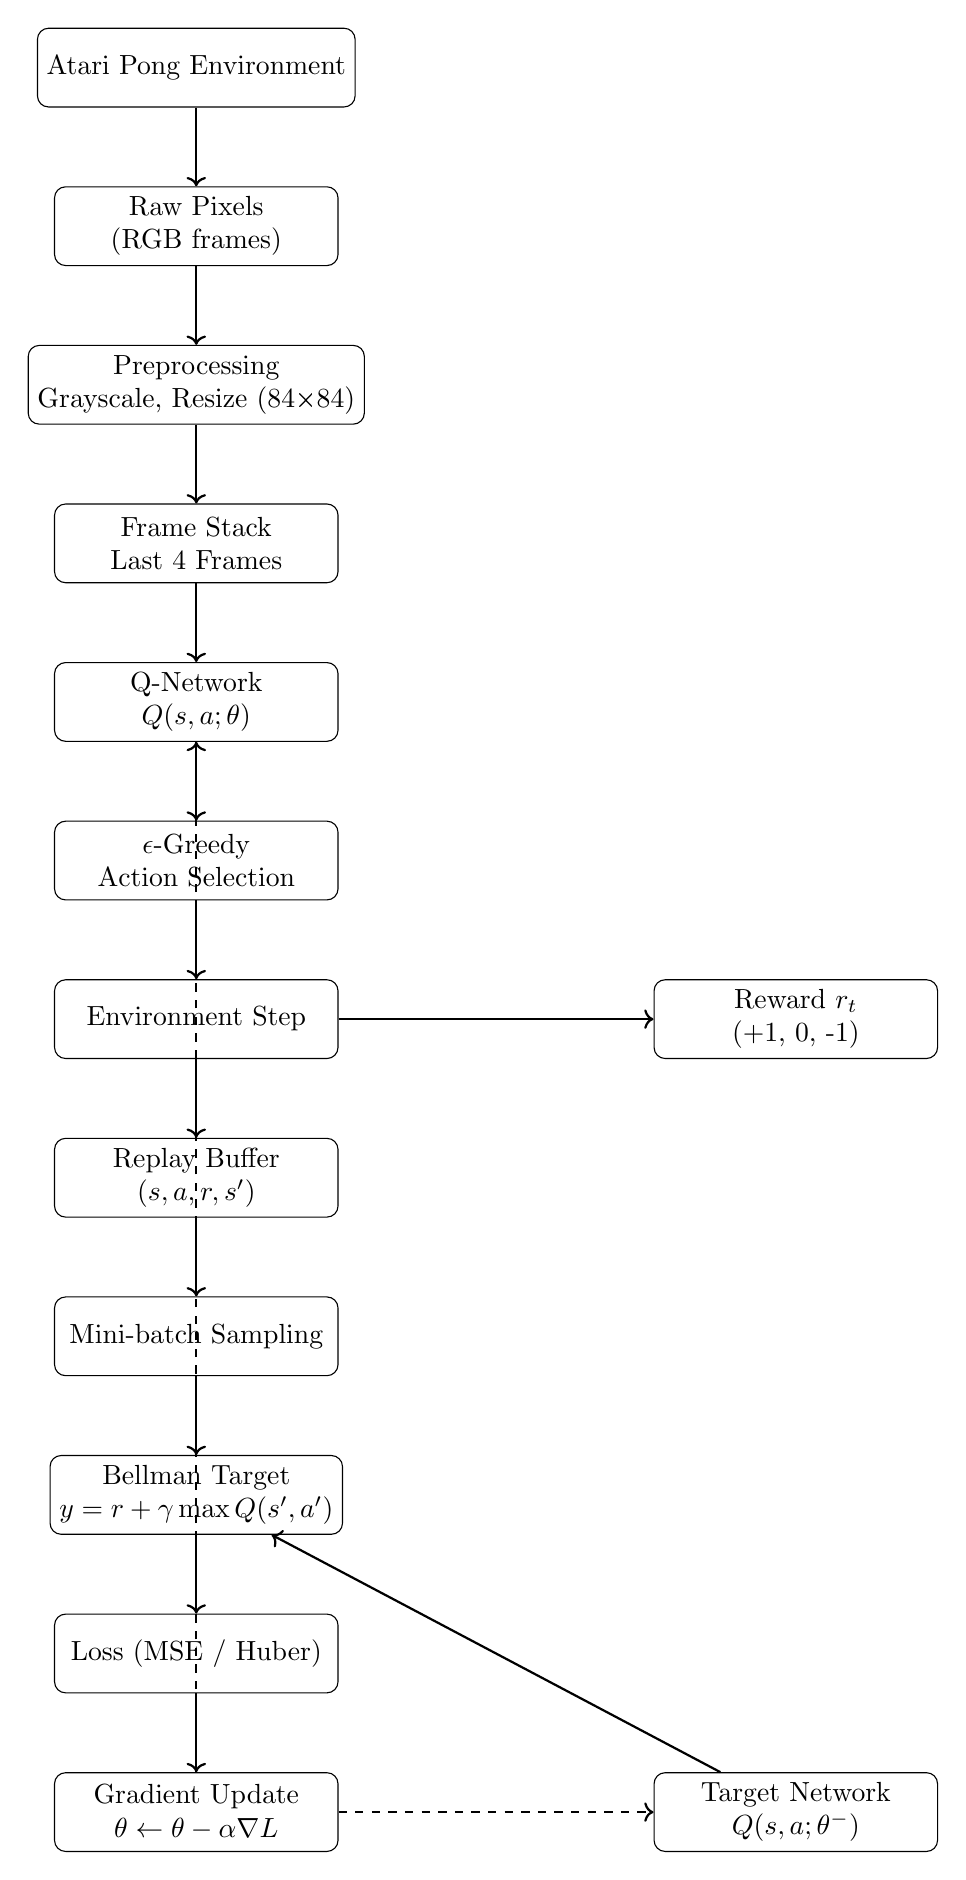
\begin{tikzpicture}[
    box/.style={draw, rectangle, rounded corners, align=center, minimum width=3.6cm, minimum height=1cm},
    arrow/.style={->, thick}
]

% Nodes
\node[box] (env) {Atari Pong Environment};
\node[box, below=of env] (pixels) {Raw Pixels\\(RGB frames)};
\node[box, below=of pixels] (preprocess) {Preprocessing\\Grayscale, Resize (84×84)};
\node[box, below=of preprocess] (stack) {Frame Stack\\Last 4 Frames};
\node[box, below=of stack] (qnet) {Q-Network\\$Q(s,a;\theta)$};
\node[box, below=of qnet] (policy) {$\epsilon$-Greedy\\Action Selection};
\node[box, below=of policy] (step) {Environment Step};
\node[box, right=4cm of step] (reward) {Reward $r_t$\\(+1, 0, -1)};
\node[box, below=of step] (replay) {Replay Buffer\\$(s,a,r,s')$};
\node[box, below=of replay] (sample) {Mini-batch Sampling};
\node[box, below=of sample] (target) {Bellman Target\\$y = r + \gamma \max Q(s',a')$};
\node[box, below=of target] (loss) {Loss (MSE / Huber)};
\node[box, below=of loss] (update) {Gradient Update\\$\theta \leftarrow \theta - \alpha \nabla L$};
\node[box, right=4cm of update] (targetnet) {Target Network\\$Q(s,a;\theta^-)$};

% Arrows
\draw[arrow] (env) -- (pixels);
\draw[arrow] (pixels) -- (preprocess);
\draw[arrow] (preprocess) -- (stack);
\draw[arrow] (stack) -- (qnet);
\draw[arrow] (qnet) -- (policy);
\draw[arrow] (policy) -- (step);
\draw[arrow] (step) -- (replay);
\draw[arrow] (replay) -- (sample);
\draw[arrow] (sample) -- (target);
\draw[arrow] (target) -- (loss);
\draw[arrow] (loss) -- (update);

\draw[arrow] (step) -- (reward);
\draw[arrow] (targetnet) -- (target);
\draw[arrow, dashed] (update) -- (qnet);
\draw[arrow, dashed] (update) -- (targetnet);

\end{tikzpicture}
}
\caption{Deep Q-Network training pipeline for Atari Pong, illustrating the flow from raw pixels to rewards and parameter updates.}
\label{fig:dqn_pong_pipeline}
\end{figure}



\end{document}
